 \documentclass[12pt]{article}
\usepackage[T2A]{fontenc}
\usepackage[utf8]{inputenc}        % Кодировка входного документа;
                                    % при необходимости, вместо cp1251
                                    % можно указать cp866 (Alt-кодировка
                                    % DOS) или koi8-r.

\usepackage[english,russian]{babel} % Включение русификации, русских и
                                    % английских стилей и переносов
%%\usepackage{a4}
%%\usepackage{moreverb}
\usepackage{amsmath,amsfonts,amsthm,amssymb,amsbsy,amstext,amscd,amsxtra,multicol}
\usepackage{verbatim}
\usepackage{tikz} %Рисование автоматов
\usetikzlibrary{automata,positioning}
\usepackage{multicol} %Несколько колонок
\usepackage{graphicx}
\graphicspath{ {images/} }
\usepackage[colorlinks,urlcolor=blue]{hyperref}
\usepackage[stable]{footmisc}

%% \voffset-5mm
%% \def\baselinestretch{1.44}
\renewcommand{\theequation}{\arabic{equation}}
\def\hm#1{#1\nobreak\discretionary{}{\hbox{$#1$}}{}}
\newtheorem{Lemma}{Лемма}
\theoremstyle{definiton}
\newtheorem{Remark}{Замечание}
%%\newtheorem{Def}{Определение}
\newtheorem{Claim}{Утверждение}
\newtheorem{Cor}{Следствие}
\newtheorem{Theorem}{Теорема}
\theoremstyle{definition}
\newtheorem{Example}{Пример}
\newtheorem*{known}{Теорема}
\def\proofname{Доказательство}
\theoremstyle{definition}
\newtheorem{Def}{Определение}



%\date{22 июня 2011 г.}
\let\leq\leqslant
\let\geq\geqslant
\def\MT{\mathrm{MT}}
%Обозначения ``ажуром''
\def\BB{\mathbb B}
\def\CC{\mathbb C}
\def\RR{\mathbb R}
\def\SS{\mathbb S}
\def\ZZ{\mathbb Z}
\def\NN{\mathbb N}
\def\FF{\mathbb F}
%греческие буквы
\let\epsilon\varepsilon
\let\es\emptyset
\let\eps\varepsilon
\let\al\alpha
\let\sg\sigma
\let\ga\gamma
\let\ph\varphi
\let\om\omega
\let\ld\lambda
\let\Ld\Lambda
\let\vk\varkappa
\let\Om\Omega
\def\abstractname{}

\def\R{{\cal R}}
\def\A{{\cal A}}
\def\B{{\cal B}}
\def\C{{\cal C}}
\def\D{{\cal D}}
\let\w\omega

%классы сложности
\def\REG{{\mathsf{REG}}}
\def\CFL{{\mathsf{CFL}}}
\newcounter{problem}
\newcounter{uproblem}
\newcounter{subproblem}
\def\pr{\medskip\noindent\stepcounter{problem}{\bf \theproblem .  }\setcounter{subproblem}{0}}
\def\prstar{\medskip\noindent\stepcounter{problem}{\bf $\theproblem^*$\negthickspace.  }\setcounter{subproblem}{0} }
\def\prpfrom[#1]{\medskip\noindent\stepcounter{problem}{\bf Задача \theproblem~(№#1 из задания).  }\setcounter{subproblem}{0} }
\def\prp{\medskip\noindent\stepcounter{problem}{\bf Задача \theproblem .  }\setcounter{subproblem}{0} }
\def\prpstar{\medskip\noindent\stepcounter{problem}{\bf Задача $\bf\theproblem^*$\negthickspace.  }\setcounter{subproblem}{0} }
\def\prdag{\medskip\noindent\stepcounter{problem}{\bf Задача $\theproblem^{^\dagger}$\negthickspace\,.  }\setcounter{subproblem}{0} }
\def\upr{\medskip\noindent\stepcounter{uproblem}{\bf Упражнение \theuproblem .  }\setcounter{subproblem}{0} }
%\def\prp{\vspace{5pt}\stepcounter{problem}{\bf Задача \theproblem .  } }
%\def\prs{\vspace{5pt}\stepcounter{problem}{\bf \theproblem .*   }
\def\prsub{\medskip\noindent\stepcounter{subproblem}{\rm \thesubproblem .  } }
\def\prsubstar{\medskip\noindent\stepcounter{subproblem}{\rm $\thesubproblem^*$\negthickspace.  } }
%прочее
\def\quotient{\backslash\negthickspace\sim}
\begin{document}
	Usvyatsov Mikhail
	
	
	\centerline{\LARGE Assignment 1}

	\bigskip
	
		\textbf{Exercises 1}		
		
		In a class of 23 students, what is the probability that at least two people have the same
birthday?
		\medskip
		
		\textbf{Solution}

		Let's estimate the probability that no one matched birthdays at the group - $\overline{p}(n)$. We can do it by fixing the random person in the group. Then we have to take the second random person in the group. Probability of the fact that birthdays are not the same is $1 - \dfrac{1}{365}$. Then let us to take the third random person. Probability of the fact that their birthdays are not the same is $1 - \dfrac{2}{365}$. E.t.c.
		
		$\overline{p}\left(n\right) = \left(1-\dfrac{1}{365}\right)\left(1-\dfrac{2}{365}\right)\left(1-\dfrac{3}{365}\right)\ldots\left(1-\dfrac{n-1}{365}\right)=\dfrac{365!}{365^n\left(365-n\right)!}$
		
		If there is 23 students at the group:
		
		$\overline{p}\left(n\right) = \dfrac{365!}{365^{23}\left(365-23\right)!}=0.4927$
		
		The probability that at least two people from the group have the same birthday is:
	
		$p\left(n\right)=1-\overline{p}\left(n\right)=0.5073$
		
		\medskip
		\textbf{Answer}: $p\left(n\right)=0.5073$
		
		
		\bigskip
		\textbf{Exercises 2}		
		
		From a group of families with two children, one family is selected. Describe the space of elementary events. Assuming all elementary events equally probable, consider the random event A: there are a boy and a girl in that family, and the random event B: there is no more than one girl in the family. Calculate $P\left(A\right)$, $P\left(B\right)$, and $P\left(A \cap B\right)$. Are the events A and B independent?
		\medskip
		
		\textbf{Solution}

We have the following space of events: two girls, two boys, the first child is a boy and the second is a girl, the first child is a girl, the second one is a boy.

		C - the probability that the child is boy is equal $\dfrac{1}{2}$.
	
		D - the probability that the child is girl is equal $\dfrac{1}{2}$.
		
		The probability of A is:
		
		$P\left(A\right) = P\left(C|D\right) + P\left(D|C\right)= \dfrac{1}{2}\cdot\dfrac{1}{2} + \dfrac{1}{2}\cdot\dfrac{1}{2} = \dfrac{1}{2}$
		
			
		$P\left(B\right) = \dfrac{1}{2}$ according to our sample space.
		
		If event A is occurred it means that there is one boy and one boy in the family. It B occurred always if A had occurred. Thus
		
		$P\left(B|A\right) = 1$
		
		Hence, 
		
		$P(A\cap B) = P\left(B|A\right)\cdot P \left(A\right) = 1 \cdot \dfrac{1}{2}=\dfrac{1}{2}$.
		
		                                                                                                                                                                                                                                                                                                                                                                                                                                                                                                                                                                                                                                                                                                                                                                                                                                                                                                                                                                                                                                                                                                                                                                                                                                                                                                                                                                                                                                                                                              		\textbf{Answer}:  A and B are not independent by definition of independence. 
		                                                                                                                                                                                                                                                                                                                                                                                                                                                                                                                                                                                                                                                                                                                                                                                                                                                                                                                                                                                                                                                                                                                                                                                                                                                                                                                                                                                                                                                                                                                                                                                                                                                                                                                                                                                                                                                                                                                                                                                                                                                                                                                                                                                                                                                                                                                                                                                                                                                                                                                                                                                                                                                                                                                                                                                                                                                                                                                                                                                     		\bigskip
		                                                                                                                                                                                                                                                                                                                                                                                                                                                                                                                                                                                                                                                                                                                                                                                                                                                                                                                                                                                                                                                                                                                                                                                                                                                                                                                                                                                                                                                                                                                                                                                                                                                                                                                                                                                                                                                                                                                                                                                                                                                                                                                                                                                                                                                                                                                                                                                                                                                                                                                                                                                                                                                                                                                                                                                                                                                                                                                                                                                
		\textbf{Exercises 3}
		
		Three fair dice are rolled. What is the probability of obtaining at least one 6 if it is known that all the three dice showed different faces?

		\medskip
		
		\textbf{Solution}
		
Let us define the requested probability p.

p = 1 - $\overline{p}$ = 1 - $\dfrac{5}{6}*\dfrac{4}{5}*\dfrac{3}{4}$ = $\dfrac{1}{2}$
		
		\medskip
		\textbf{Answer}: $p = \dfrac{1}{2}$
		
		\bigskip
		
		\textbf{Exercises 4}
		
Suppose a breathalyzer has $5\%$  false positives and $8\%$ false negatives. That is, only $5\%$ of the time will it indicate that a person is drunk when he is actually sober and $8\%$ of the time will it indicate that a person is sober when the person is in fact drunk. Using this test, the police spot test a population of drivers, $99\%$ of whom are sober.
What is the chance that a person, who tests as drunk, is actually sober?

		\medskip
		
		\textbf{Solution}

		$p\left(D\right)$ - the probability the test shows that a person is is drunk:
		
		$p\left(D\right) = p\left(D|drunk\right)\cdotp p \left(drunk\right)+p\left(D|sober\right)\cdot p\left(sober\right) =$
		
$\left(1-0.08\right)\cdot 0.01+0.05\cdot 0.99 = 0.0587$
		
		According to Bayes' rule:
		
		$p\left(D\right)=\dfrac{p(D|sober)\cdot p\left(sober\right)}{p\left(D\right)}=\dfrac{0.05\cdot 0.99}{0.0587}=0.84327$
		
		\medskip
		\textbf{Answer}: $p\left(D\right) = 0.843$
		
		\bigskip
		
		\textbf{Exercises 5}
		
		Two fair dice are rolled. Let $X_1$ denote the number of points shown by the first die and $X_2$ denote the number of points shown by the second die. Consider the following events:
		
$A_1$ = $\left\lbrace X_1\ is\ divisible\ by\ 2,\ X_2\ is\ divisible\ by\ 3 \right\rbrace$

$A_2$ = $\left\lbrace X_1\ is\ divisible\ by\ 3,\ X_2\ is\ divisible\ by\ 2 \right\rbrace$

$A_3$ = $\left\lbrace X_1\ is\ divisible\ by\ X_2 \right\rbrace$

$A_4$ = $\left\lbrace X_2\ is\ divisible\ by\ X_1 \right\rbrace$

$A_5$ = $\left\lbrace X_1\ +\ X_2\ is\ divisible\ by\ 2 \right\rbrace$

$A_6$ = $\left\lbrace X_1\ +\ X_2\ is\ divisible\ by\ 3 \right\rbrace$
		
		\medskip
		
		\textbf{Solution}

It is obvious that:
\medskip		

P$\left(A_1\right)$ = $\dfrac{1}{6}$
P$\left(A_2\right)$ = $\dfrac{1}{6}$
P$\left(A_3\right)$ = $\dfrac{7}{18}$
P$\left(A_4\right)$ = $\dfrac{7}{18}$
P$\left(A_5\right)$ = $\dfrac{1}{2}$
P$\left(A_6\right)$ = $\dfrac{1}{3}$
\medskip

So let's find all jointly probabilities
\medskip

\begin{table}[h]
\begin{tabular}{llllll}
P$\left(A_1 \cap A_2\right)$ = $\dfrac{1}{36}$  & P$\left(A_2 \cap A_3\right)$ = $\dfrac{1}{18}$ & P$\left(A_3 \cap A_4\right)$ = $\dfrac{1}{6}$ & P$\left(A_4 \cap A_5\right)$ = $\dfrac{1}{4}$ & P$\left(A_5 \cap A_6\right)$ = $\dfrac{1}{6}$ \\[7pt]
P$\left(A_1 \cap A_3\right)$ = $\dfrac{1}{36}$  & P$\left(A_2 \cap A_4\right)$ = $\dfrac{1}{18}$ & P$\left(A_3 \cap A_5\right)$ = $\dfrac{1}{4}$ & P$\left(A_4 \cap A_6\right)$ = $\dfrac{1}{6}$ \\[7pt]
P$\left(A_1 \cap A_4\right)$ = $\dfrac{1}{36}$  & P$\left(A_2 \cap A_5\right)$ = $\dfrac{1}{36}$ & P$\left(A_3 \cap A_6\right)$ = $\dfrac{1}{6}$ &  \\[7pt]
P$\left(A_1 \cap A_5\right)$ = $\dfrac{1}{36}$  & P$\left(A_2 \cap A_6\right)$ = $\dfrac{1}{36}$ &  &  \\[7pt]
P$\left(A_1 \cap A_6\right)$ = $\dfrac{1}{36}$  &  &  &
\end{tabular}
\end{table}				

		\medskip
		\textbf{Answer}:	
			
By definition of independence only 		
$\left\lbrace A_1\ and\ A_2 \right\rbrace$,
$\left\lbrace A_5\ and\ A_6 \right\rbrace$ are independent.

There is no reason to check triples and another combinations because it will include not independent events and so will not be independent.
		
		\bigskip

		
		\textbf{Exercises 6}

A)  Let X be a random variable with a uniform distribution, i.e. with pdf equal to 1 for
x $\in$ [0, 1] and 0 otherwise. Find the pdf of Y = exp(tX) for a fixed t. (This transformation is known as the moment generation function)

B) Find the pdf for this transformation (exp(t*x)) if the pdf of X is equal to exp(-x) for x positive and 0 otherwise.
		
		\medskip
		
		\textbf{Solution}
		
According to the theorem from George Casella book
\medskip

$f_y(y)$ = $f_x(g^{-1}(y))$ * $\dfrac{g^{-1}(y)}{dy}$ if g(x) increases
\medskip

$f_y(y)$ = -$f_x(g^{-1}(y))$ * $\dfrac{g^{-1}(y)}{dy}$ if g(x) decreases
\medskip

A) 
\medskip

\[f_x(x) = \left\{
\begin{array}{l l}
  1,\ x \in [0, 1]\\
  0\ otherwise
\end{array} \right.\]
\medskip

x $\in$ [0, 1] so 
y $\in$ [1, $e^t$]
\medskip

g(x) = $e^{tx}$	
\medskip

$g^{-1}(y)$ = $\dfrac{ln(y)}{t}$
\medskip

$\dfrac{g^{-1}(y)}{dy}$ = $\dfrac{1}{ty}$
\medskip

$f_y(y)$ = $\dfrac{1}{ty}$
\medskip

B)
\medskip

\[f_x(x) = \left\{
\begin{array}{l l}
  e^{-x},\ x > 0\\
  0\ otherwise
\end{array} \right.\]
\medskip

g(x) = $e^{tx}$	
\medskip

$g^{-1}(y)$ = $\dfrac{ln(y)}{t}$
\medskip

$\dfrac{g^{-1}(y)}{dy}$ = $\dfrac{1}{ty}$
\medskip

$f_y(y)$ = $e^{-\dfrac{ln(y)}{t}}$ * $\dfrac{1}{ty}$
\medskip


		\medskip
		\textbf{Answer}:

A)
\medskip

\[f_y(y) = \left\{
\begin{array}{l l}
  \dfrac{1}{ty}, y \in [1, e^t]\\
  0\ otherwise
\end{array} \right.\]

B)
\medskip

\[f_y(y) = \left\{
\begin{array}{l l}
  \dfrac{y^{-\dfrac{1}{t}-1}}{t}, x > 0\\
  0\ otherwise
\end{array} \right.\]
		

		
		\bigskip
		
		\bigskip
		
		\textbf{Exercises 7}		
		\medskip

The random variable X has an exponential distribution:
$F_x(x)$ = P(X<x) = 1 - $e^{-x}$, (x > 0). What is the pdf $f_x$ of X? Find the probability density functions of the following random variables:
\medskip

\newcounter{fcounter}
\begin{list}{\alph{fcounter}) ~}{\usecounter{fcounter}}
	\item $Y_1$ = $\sqrt{X}$
	\item $Y_2$ = $X^2$
	\item $Y_3$ = ln(X)
	\item $Y_4$ = $\dfrac{1}{X}$
	\item $Y_5$ = 1 - $e^{-X}$
	\item Simulate 10000 draws of the random variable X: Use a histogram to show that the
simulated X has the pdf $f_X(x)$
	\item Use the simulated X to generate 10000 draws of the random variable $Y_1$ = $\sqrt{X}$.
Use a histogram for simulated $Y_1$ to show that your answer to (a) is correct.
\end{list}
		
\textbf{Solution}
\medskip

$F_x(X)$ = P(X$\leq$ x) = 1 - $e^{-x}$,
x $\geq$ 0
\medskip

$f_x(x)$ = $e^{-x}$
\bigskip

\newcounter{gcounter}
\begin{list}{\alph{gcounter}) ~}{\usecounter{gcounter}}
	\item $Y_1$ = $\sqrt{X}$

		$g^{-1}(y)$ = $y^2$

		$\dfrac{g^{-1}(y)}{dy} = 2y$
		
		$f_y(y)$ = $f_x(g^{-1}(y)) * \dfrac{g^{-1}(y)}{dy}$ = $e^{-y^2} * 2y$

\[f_y(y) = \left\{
\begin{array}{l l}
  e^{-y^2} * 2y, y \geq 0\\
  0\ otherwise
\end{array} \right.\]

		\item $Y_2$ = $X^2$
		
		$F_y(y) = P(-\sqrt{y} \leq X \leq \sqrt{y} ) = P(-\sqrt{y} < X \leq \sqrt{y} ) = P(x \leq \sqrt{y}) - P(x\leq-\sqrt{y}) = F_x(\sqrt{y}) - F_x(-\sqrt{y}) = e^{\sqrt{y}} - e^{-\sqrt{y}}$

		$f_y(y)$ = $\dfrac{ e^{\sqrt{y}}+e^{-\sqrt{y}} }{2\sqrt{y}}$

\[f_y(y) = \left\{
\begin{array}{l l}
  \dfrac{ e^{\sqrt{y}}+e^{-\sqrt{y}} }{2\sqrt{y}}, y \geq 0\\
  0\ otherwise
\end{array} \right.\]

		\item $Y_3 = ln(X)$

		$g^{-1}(y) = e^y$

		$\dfrac{g^{-1}(y)}{dy} = e^y$

		$f_y(y) = f_x(g^{-1}(y)) * \dfrac{g^{-1}(y)}{dy} = e^{-e^y} * e^y$

		\item $Y_4 = \dfrac{1}{X}$

			$g^{-1}(y) = \dfrac{1}{y}$

			$\dfrac{g^{-1}(y)}{dy} = - \dfrac{1}{y^2}$

			$f_y(y) = - f_x(g^{-1}(y)) * \dfrac{g^{-1}(y)}{dy} = \dfrac{e^{-\dfrac{1}{y}}}{y^2}$

\[f_y(y) = \left\{
\begin{array}{l l}
  \dfrac{e^{-\dfrac{1}{y}}}{y^2}, y \geq 0\\
  0\ otherwise
\end{array} \right.\]

		\item $Y_5 = 1 - e^{-X}$

		$g^{-1}(y) = - ln(1 - y)$


		$\dfrac{g^{-1}(y)}{dy} = \dfrac{1}{1-y}$

		$f_y(y) = - f_x(g^{-1}(y)) * \dfrac{g^{-1}(y)}{dy} = 1$

\[f_y(y) = \left\{
\begin{array}{l l}
  1, y \in [0,1]\\
  0\ otherwise
\end{array} \right.\]

		\item Using Inverse transform sampling we can get random variable distributed by the given low, using uniform distributed variable for generation.

$Y = - ln(1 - X)$, $X \in N[0,1]$

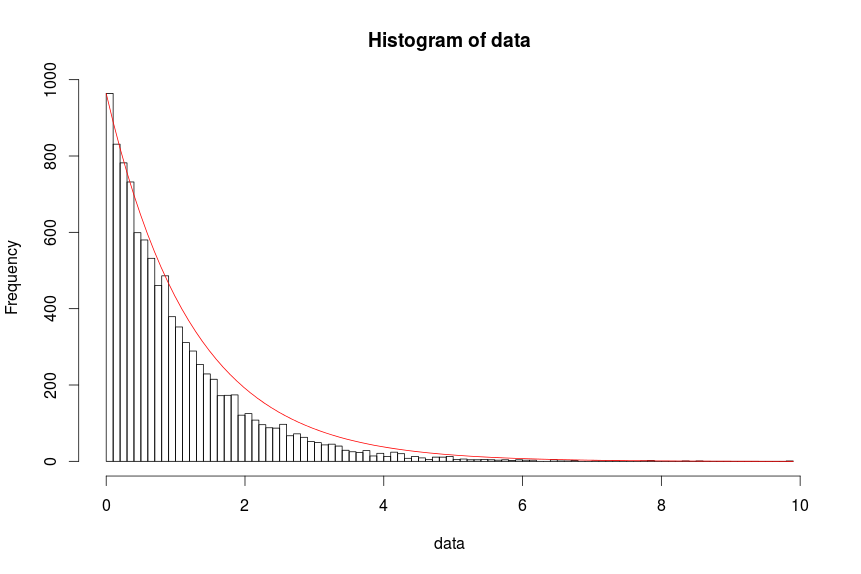
\includegraphics[width=1\textwidth]{Rplot.png}

		\item Using Inverse transform sampling we can get random variable distributed by the given low, using uniform distributed variable for generation.
		{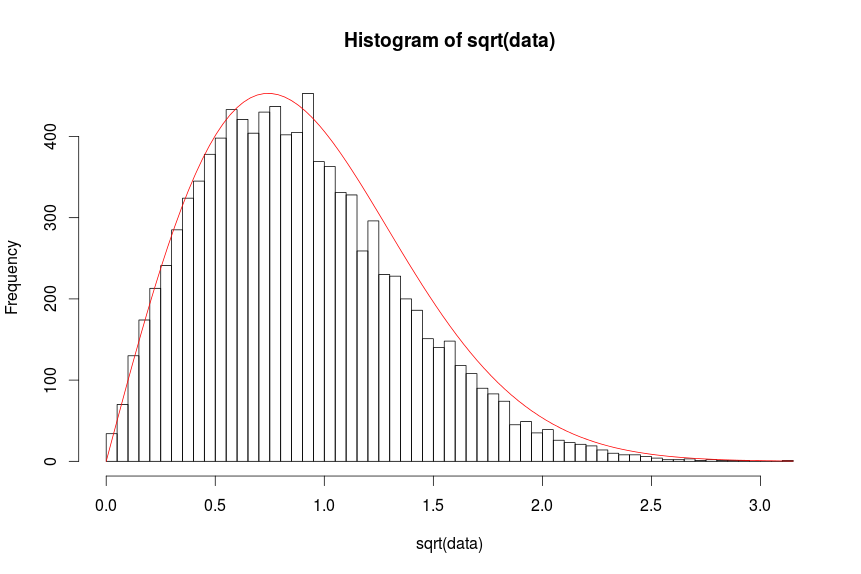
\includegraphics[width=1\textwidth]{Rplot01.png}}

\end{list}
		\medskip
		\textbf{Answer}:

		\bigskip
		\textbf{Exercises 8}

		The pdf of a random vector $(X, Y)$ is 
		
$f_{X,Y}\left(x, y\right) = 24x^2 y\left(1-x\right)$, $0<x<1$, $0<y<1$ and $f_{X,Y}\left(x, y\right) = 0$ otherwise. Find
\newcounter{qcounter}
\begin{list}{\alph{qcounter}) ~}{\usecounter{qcounter}}
\item The pdf and cdf of X;
\item The pdf and cdf of Y ;
\item Are the random variables X and Y independent?
\end{list}
		\medskip
		
		\textbf{Solution}
\newcounter{bcounter}
\begin{list}{\alph{bcounter}) ~}{\usecounter{bcounter}}		
		\item $f_X(x) = \int_{-\infty}^{\infty} f_{X,Y}(x,y)dy = \int_0^1 24x^2 y\left(1-x\right)dy=-12\left(1-x\right)x^2$
		
		\item $f_Y(y) = \int_{-\infty}^{\infty} f_{X,Y}(x,y)dx = \int_0^1 24x^2 y\left(1-x\right)dx=2y$
		
		\item According to the Lemma 4.2.7 from "Statistical Inference"    \ the X and Y are independent if:
		
		$f(x,y) = g(x)h(y)$
		
		Hence, 
		
		$f_X(x)f_Y(y) = -12\left(1-x\right)x^2 \cdot 2y = -24x^2 y\left(1-x\right)$
		
		$f_X(x)f_Y(y) \neq f_{X, Y}$ - X and Y are depend
		
\end{list}

		\medskip
		\textbf{Answer}:		
\newcounter{ccounter}
\begin{list}{\alph{ccounter}) ~}{\usecounter{ccounter}}			
		\item $f_X(x)= -12\left(1-x\right)x^2$;
		
		\item $f_Y(y) =2y$;
		
		\item X and Y are dependent.
\end{list}

\end{document}
